\newpage
\appendix
\onecolumn

\section{Verifier Prompt and Additional Analysis}
\label{app:verifier}

\subsection{Verifier Prompt Template}
\label{app:verifier_prompt}

Given the current state $s_t$ and a draft output consisting of an optional reasoning trace $z_t$ and a candidate action $a_t$, we query the large model as a critic to output a binary judgment (\texttt{Yes} or \texttt{No}).
The critic is instructed to jointly assess (i) whether the trajectory is making new progress toward the user goal and (ii) whether the proposed action is grounded and useful.
When the draft pathway skips explicit reasoning, we set $z_t=\emptyset$.
The exact prompt used for the critic is shown below.

\begin{quote}
\small
\noindent\textbf{[SYSTEM: TRAJECTORY AUDIT]}\\
Review the recent steps (context). Is the agent making \textbf{NEW PROGRESS}?\\[0.3em]
\noindent\textbf{REJECT ("No") if:}
\begin{enumerate}
    \item \textbf{Stagnation}: Repeating similar queries or visiting same URLs (Looping).
    \item \textbf{Ungrounded Answer}: The Final Answer is NOT supported by the \textit{retrieved search results}.
    \item \textbf{Lazy/Drift}: Queries are nested, vague, or irrelevant to User's Goal.
\end{enumerate}
\noindent Verdict: Is the trajectory HEALTHY and PROGRESSING?\\
Answer only "Yes" or "No".
\end{quote}

\subsection{Verifier Score Distributions}
\label{app:verifier_scores}

To further validate that the verifier score provides a meaningful signal, we analyze the score distributions on complete trajectories.
Specifically, we apply two full-size critics, MiroThinker-72B and Qwen3-32B, to evaluate step-level draft outputs produced by MiroThinker-8B and Qwen3-4B, respectively.
We report two aggregated statistics per trajectory: the mean score across all steps (\texttt{Mean}) and the 25th percentile score (\texttt{p25}), where \texttt{p25} emphasizes low-confidence segments within a trajectory.

\begin{figure}[H]
    \centering
    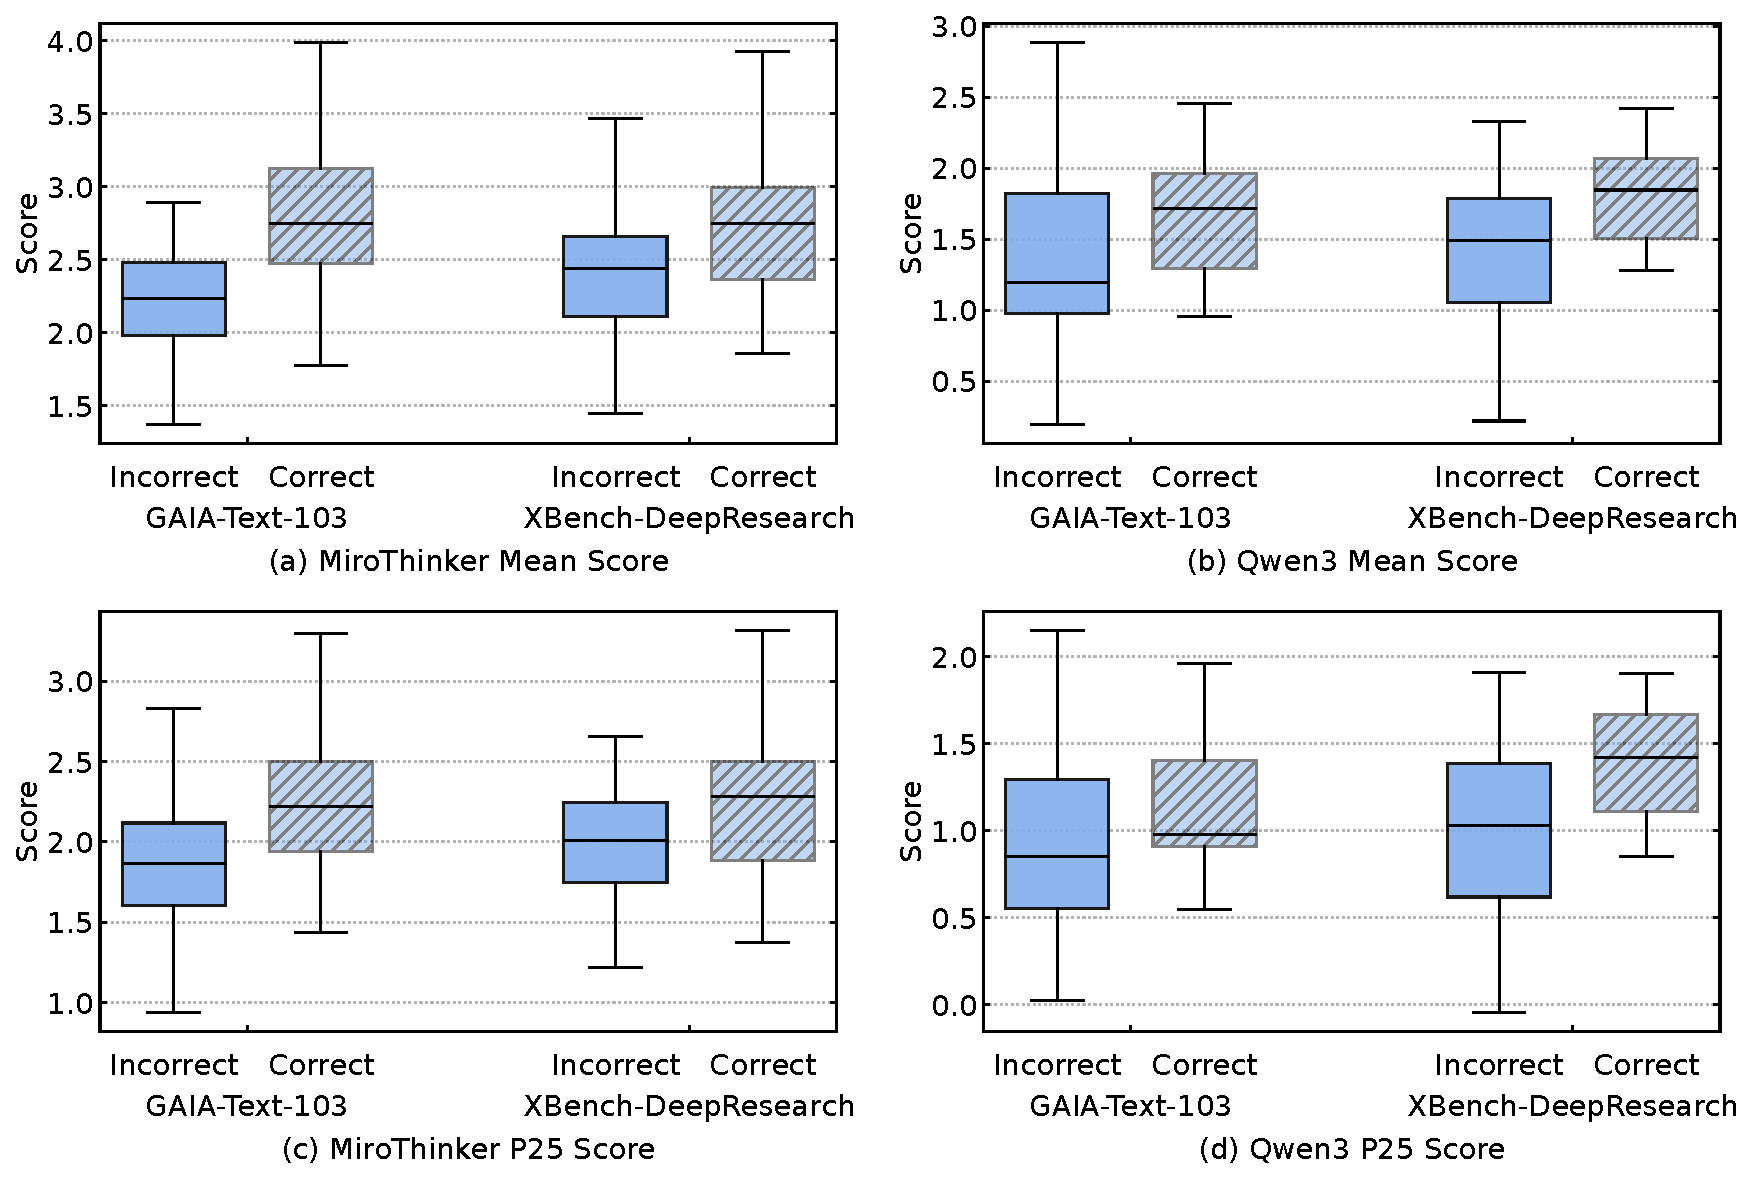
\includegraphics[width=0.8\linewidth]{figs/score.pdf}
    \caption{Verifier score distributions on GAIA and XBench-DeepResearch.
    We report trajectory-level aggregated verifier scores for (a) MiroThinker mean score, (b) Qwen mean score,
    (c) MiroThinker p25 score, and (d) Qwen p25 score.
    Correct trajectories consistently receive higher scores than incorrect ones, suggesting that the verifier provides a useful reliability signal.}
    \label{fig:verifier_score_dist}
\end{figure}

Figure~\ref{fig:verifier_score_dist} shows the score distributions on GAIA and XBench-DeepResearch, grouped by whether the final answer is correct.
Across both datasets and both model families, correct trajectories consistently exhibit higher verifier scores than incorrect ones under both \texttt{Mean} and \texttt{p25}.
This indicates that the verifier score correlates with end-to-end task success, supporting its use as a lightweight reliability signal for controlling speculative execution.


